%!TEX root = ../scivis_lbaakman_bvanloon.tex
In this section the main methods for color mapping are discussed. In \cref{sub:texture_mapping} we discuss \emph{texture mapping}, the method used to map scalar values to colors. Next \cref{ss:colormaps:parameterization} considers the parametrization of color maps and explains how the number of colors and the saturation can influence the quality of a color map. Last \cref{ss:colormaps:applying} shows how color maps are applied to scalar data.

\subsection{Texture Mapping} % (fold)
\label{sub:texture_mapping}
To implement the color maps \emph{texture mapping} is used. The general pipeline of texture mapping is as follows. First the scalar values are sampled for each vertex in the simulation grid. Next the vertices of the triangulation of the simulation grid are passed to the vertex shader with the associated scalar values. The vertex shader normalizes scalar values associated with the vertices using a given range of the scalar values creating texture-coordinates for every vertex. This step ensures that the texture coordinates are in the range [0, 1]. The texture-coordinates are passed to the fragment shader and are automatically interpolated by OpenGL. The fragment shaders retrieves the color that is associated with the texture coordinate it receives.

The end result is a piecewise-linear reconstruction of the scalar field. By interpolating the texture coordinates, interpolation of colors is prevented.  This ensures that no false colors are displayed in the visualization. This is also the main motivation for the choice of texture mapping. The alternative, naive, method of vertex-based color mapping can result in colors that do not correspond with the actual scalar values or worse, colors that are not in the color map. These problems are prevented by avoiding the interpolation of colors. 

Since we use texture mapping a color map is defined as a 1D texture that represents the range o colors that are associated with the scalar values normalized to the range [0, 1]. Defining color maps as 1D image, has the added advantage of making the definition of new color maps trivial, as evidenced by the large number of color maps supported by our application.

\subsection{Parameterization of Color Maps}
\label{ss:colormaps:parameterization}
Given a color map scheme there are two parameters which can influence the final map. The number of colors in the color map and the saturation of the colors, these parameters are discussed in \cref{ssub:number_of_colors} and \cref{ssub:saturation}, respectively. 

\subsubsection{Number of Colors} % (fold)
\label{ssub:number_of_colors}
The number of colors influences how smooth the color map is perceived to be. When the number of colors in a color map is low, there is a relatively large difference between the scalar values associated with two neighboring colors in the color map. In the visualization this large step shows up as sharp edges between areas with different scalar values. An example of this banding effect is given in \cref{fig:colormaps:banding} which shows the difference between two color maps that use the same color scheme, but a different number of colors. We observe that \cref{fig:colormapping:banding:20} shows distinct bands of colors, whereas \cref{fig:colormapping:banding:256} has smooth transitions between the colors. In our application the user can select the desired number of colors form the range [2, 256]. The default value is set to 256 colors to ensure a smooth color map. Using a color map with fewer colors would introduce sharp transitions in the visualization that are not present in the data. 
%
\begin{figure}[tb]
	\centering
	\begin{subfigure}[t]{0.4\textwidth}
		\centering
		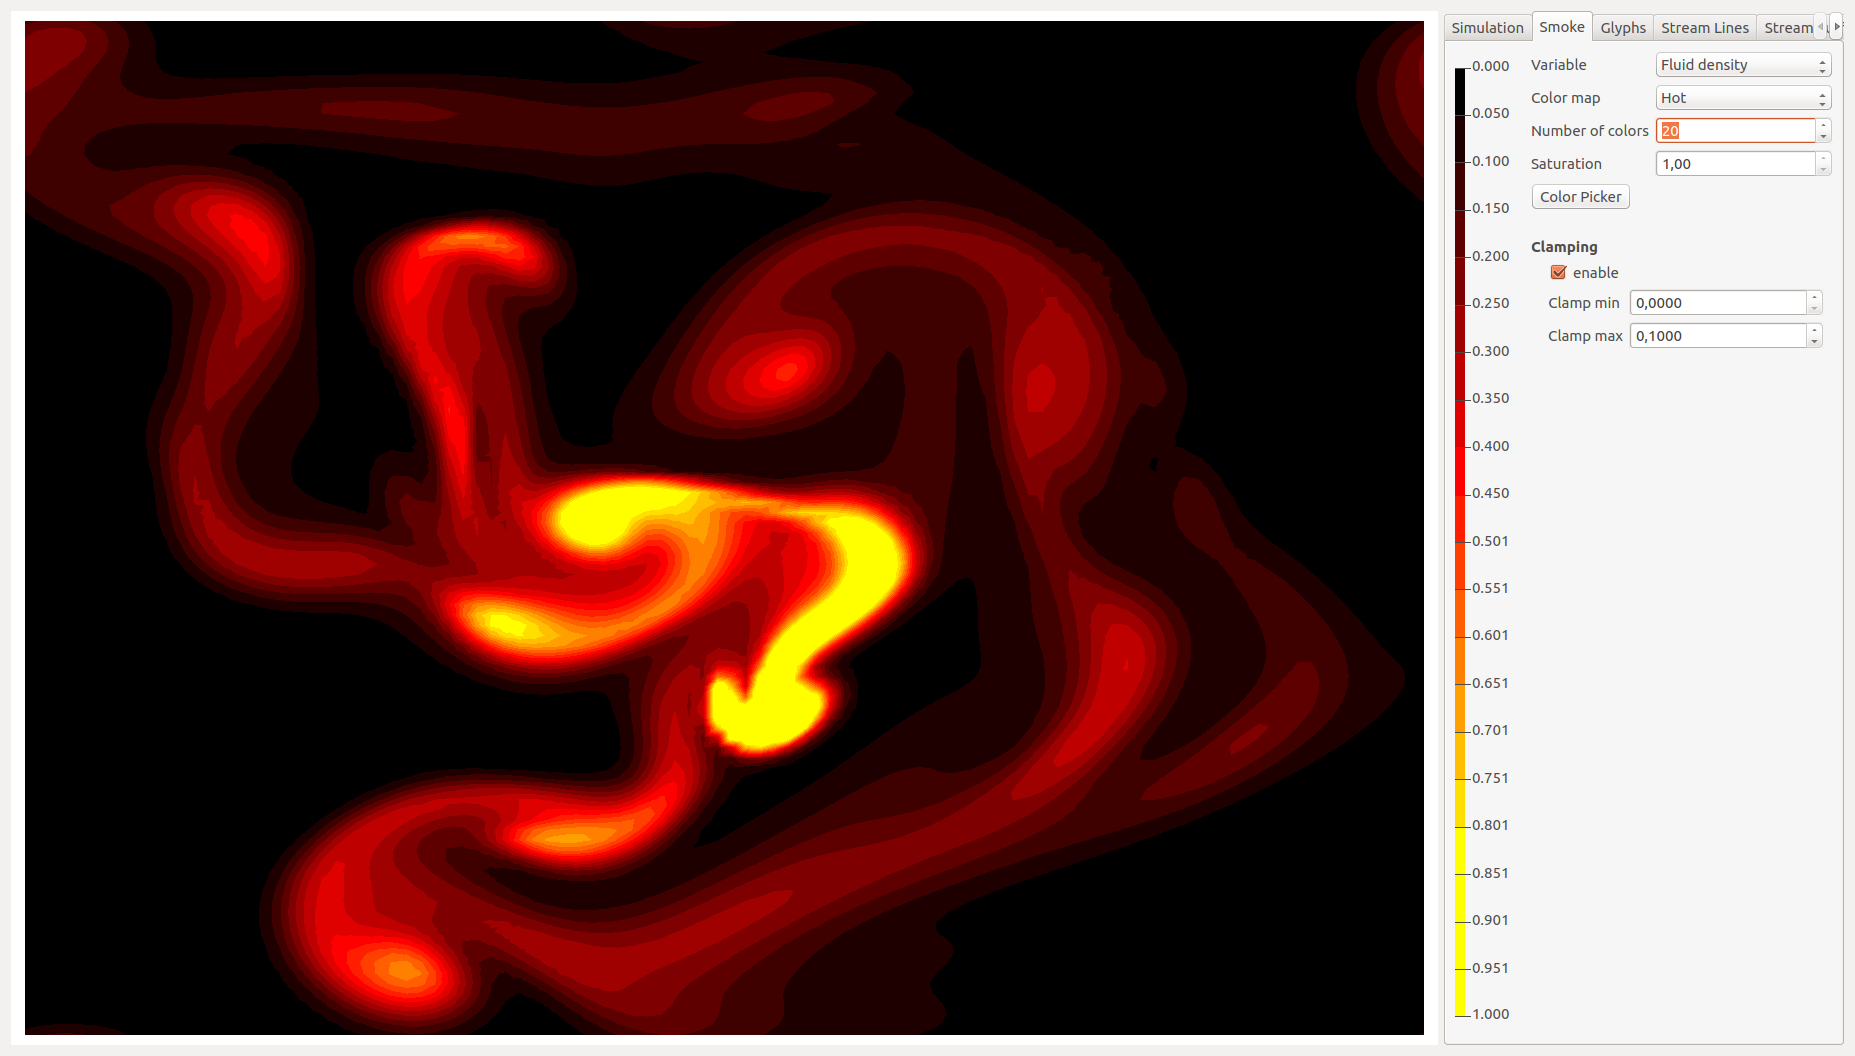
\includegraphics[width=\textwidth, trim={235px 30px 1230px 830px}, clip]{colormapping/img/heat20}
		\caption{Example of a visualization using a heat-map containing 20 colors.}
		\label{fig:colormapping:banding:20}
	\end{subfigure}
	\hspace{50px}
	\begin{subfigure}[t]{0.4\textwidth}
		\centering
		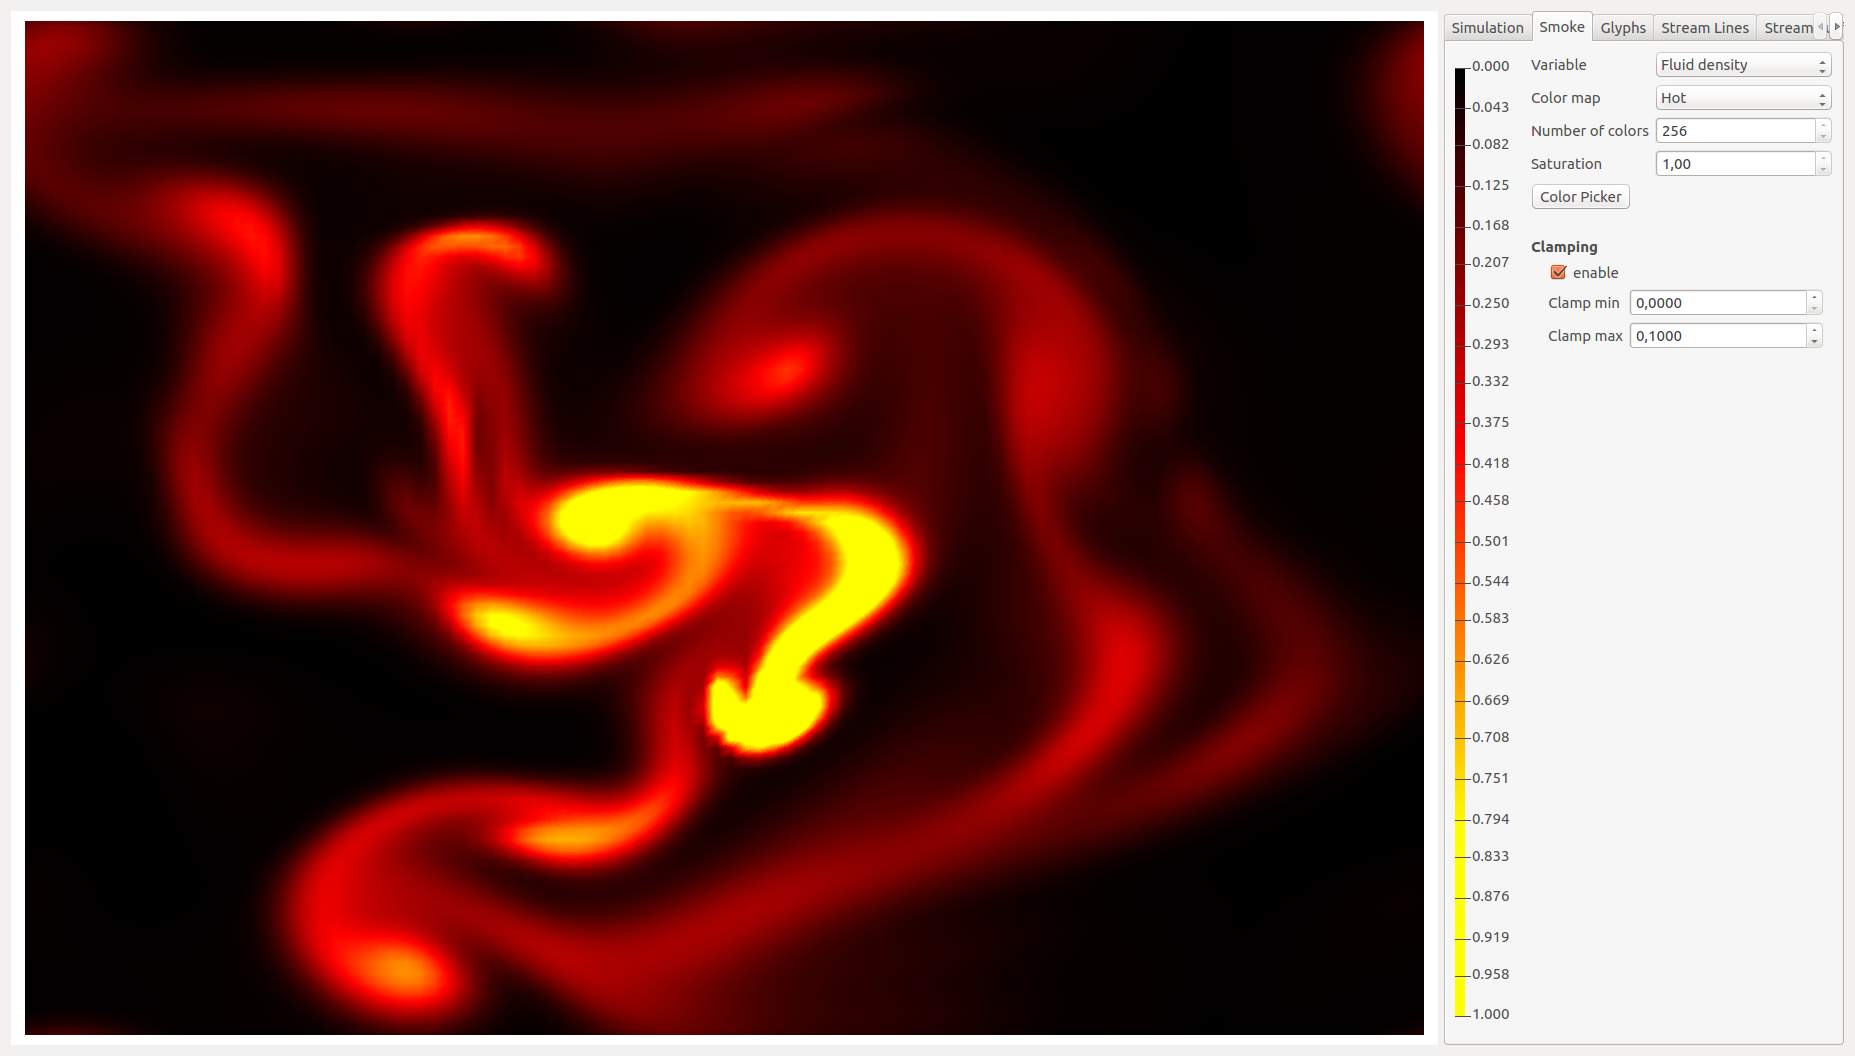
\includegraphics[width=\textwidth, trim={235px 30px 1230px 830px}, clip]{colormapping/img/heat256}
		\caption{Example of a visualization using a heat-map containing 256 colors.}
		\label{fig:colormapping:banding:256}
	\end{subfigure}	
	\caption{The influence of the number of colors in the color map shown, using the heat-map using \subref{fig:colormapping:banding:20} 20 and \subref{fig:colormapping:banding:256} 256 colors. Both images are taken from the same simulation state and zoomed in on the same location.}
	\label{fig:colormaps:banding}
\end{figure}

\subsubsection{Saturation} % (fold)
\label{ssub:saturation}
Besides the number of colors it is also possible to change the saturation of a subset of the color maps. Saturation influences the intensity of a color: colors with full saturation will appear pure, whereas colors with low saturation appear more washed out. Changing the saturation of a color map can be of use when displaying multiple visualization techniques together. An example of the effect of changing saturation is given in \cref{fig:colormaps:saturation}. In \cref{fig:colormapping:saturation:disabled} the glyphs are almost non distinguishable from the scalar visualization, their visibility is greatly enhanced in \cref{fig:colormapping:saturation:enabled}, which uses a color map with a lower saturation. In the application it is possible to change the saturation of most color maps, however the user should keep in mind that lowering the saturation can cause a less distinct ordering of the colors in the color map.

\begin{figure}[tb]
	\centering
	\begin{subfigure}[t]{0.4\textwidth}
		\centering
		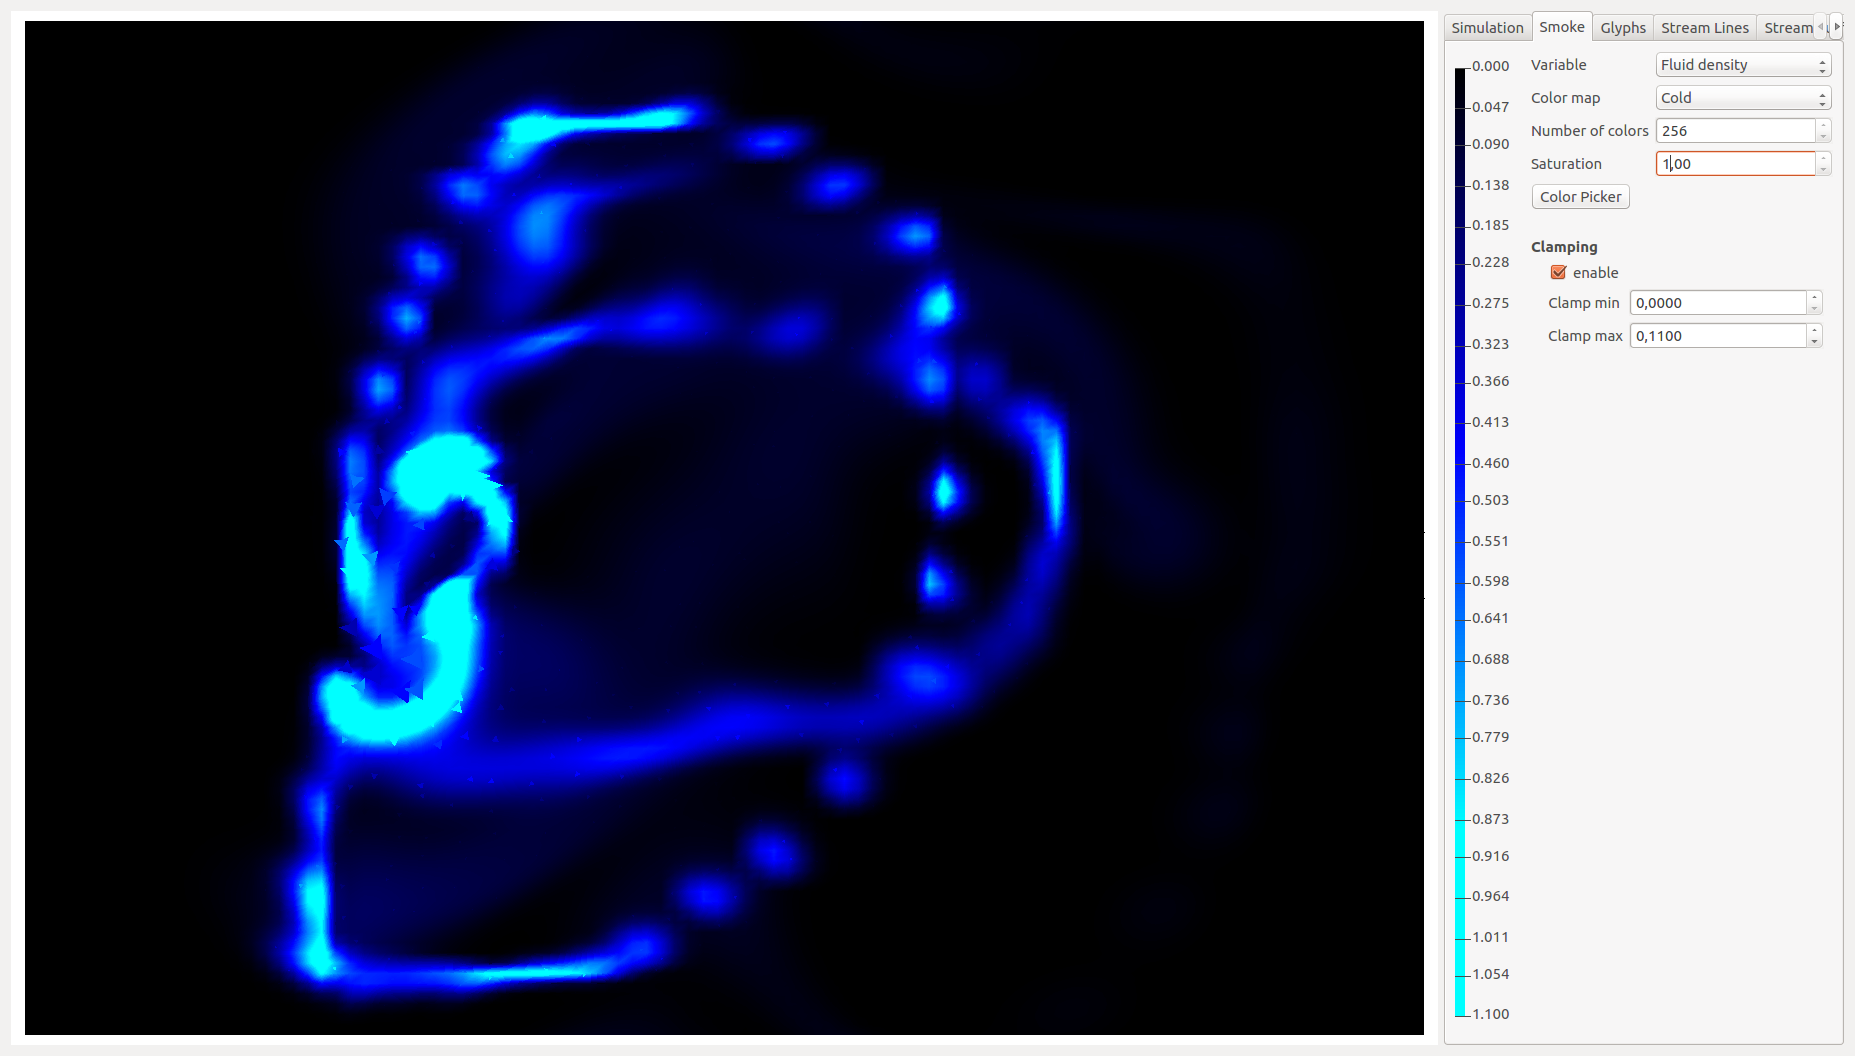
\includegraphics[width=\textwidth, trim={50px 200px 1023px 300px}, clip]{colormapping/img/nosaturation}
		\caption{scalar visualization saturation = 1.0}
		\label{fig:colormapping:saturation:disabled}
	\end{subfigure}
	\hspace{50px}
	\begin{subfigure}[t]{0.4\textwidth}
		\centering
		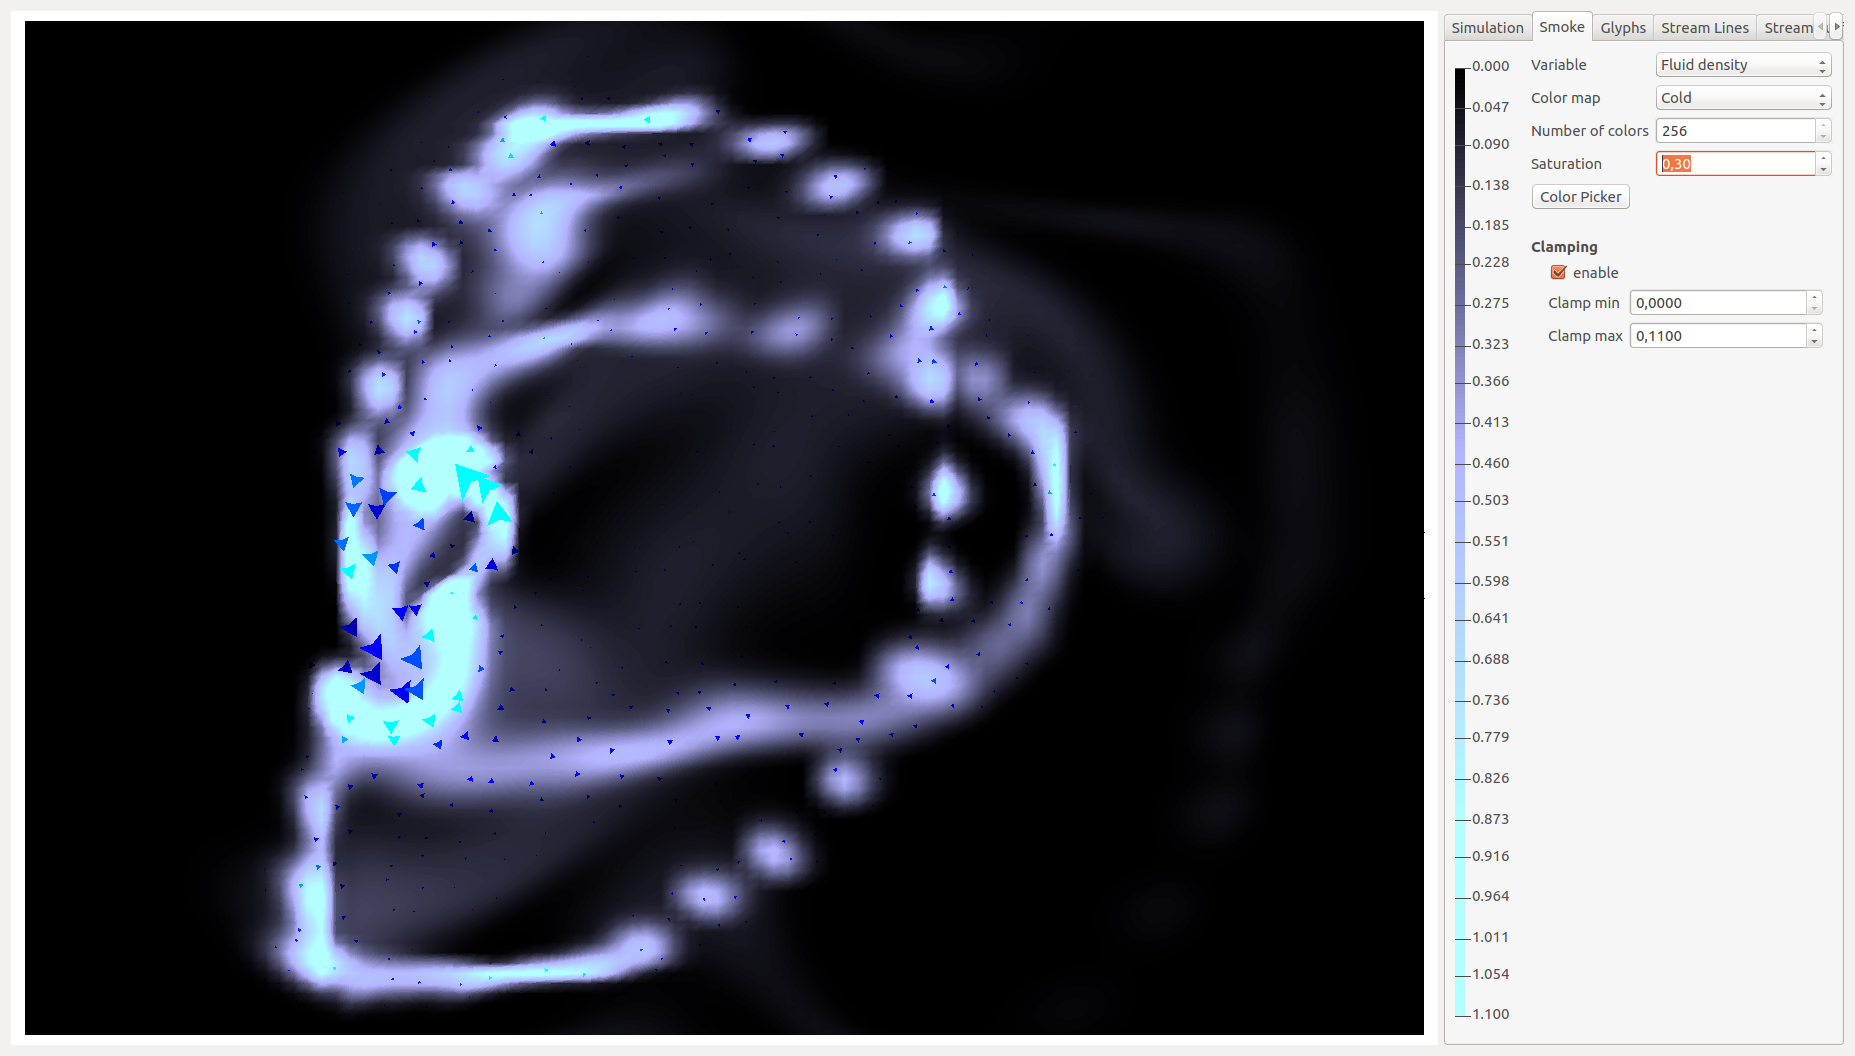
\includegraphics[width=\textwidth, trim={50px 200px 1023px 300px}, clip]{colormapping/img/saturation}
		\caption{scalar visualization saturation = 0.30}
		\label{fig:colormapping:saturation:enabled}
	\end{subfigure}	
	\caption{An illustration of the influence of saturation when combining \smoke and vector visualization. The vector visualization is fully saturated in both images, the color map used for the scalar visualization is \subref{fig:colormapping:saturation:disabled} fully saturated, and \subref{fig:colormapping:saturation:enabled} partially saturated.}
	\label{fig:colormaps:saturation}
\end{figure}

\subsection{Applying Colormaps}
\label{ss:colormaps:applying}
An important aspect of using color maps is how they are applied to the scalar values. Given a color map of $N$ colors with colors $c_1,c_2,\cdots,c_N$ and scalars in the range $[f_{\text{min}}, f_{\text{max}}]$ each scalar values is mapped to a color via linear scaling. The choice of $[f_{\text{min}}, f_{\text{max}}]$ is important when using a color map. Imagine that we have picked $f_{\text{min}} = 0$ and $f_{\text{max}} = 100$ but the actual range of the scalar values in the simulation is between $10$ and $20$. In this case the visualization would only use one out of ten colors present in the color map. Ideally the entire range of the color map is applied to the full range of scalar values.

In our application $[f_{\text{min}}, f_{\text{max}}]$ can be set in two ways. The first method uses a fixed range of $f_{\text{min}} = 0$ and picks $f_{\text{max}}$ based on the scalar value visualized and the forces that are input by the user\footnote{Given an input force set to 10 we have (empirically) determined that the fluid density has $f_{\text{max}} = 10$, fluid velocity magnitude has $f_{\text{max}} = 0.1$, and the force field magnitude has $f_{\text{max}} = 0.1$.}. These $[f_{\text{min}}, f_{\text{max}}]$ are initialized as such, however the user can update these fixed ranges based on the current dynamic range. These fixed ranges allow the user to observe the change in the scalar field as a function of time. The disadvantage is that after some time in which no new forces are added to the simulation, the range of the scalar values only uses a small subset of the color map. Which makes it hard to observe the differences between scalar values.

The second method uses a dynamic range $[f_{\text{min}}, f_{\text{max}}]$. This is done by determining the minimum and maximum of the all scalar fields for every time-step in the simulation and updating $[f_{\text{min}}, f_{\text{max}}]$ accordingly. The advantage of this approach is that at every time-step the full range of the color map is used. But it hides the changes of the scalar field as s function of time.

\subsubsection{Clamping} % (fold)
\label{ssub:clamping}
Previously we assumed that the scalar values were uniformly distributed. However, some simulations might result in non-uniformly distributed scalar values, \eg most scalar values fall within a range much smaller than $[f_{\text{min}}, f_{\text{max}}]$. In these cases it might be desirable to show more detail in the range that contains the most scalar values. To facilitate this the user can adapt $[f_{\text{min}}, f_{\text{max}}]$ to a range $[f^{clamp}_{min}, f^{clamp}_{max}]$ such that $f_{\text{min}} \leq f^{clamp}_{min}$ and $f_{\text{max}} \geq f^{clamp}_{max}$\footnote{At all times it is ensured that $f^{clamp}_{max} > f^{clamp}_{min}$ }. Scalar values outside the range $[f^{clamp}_{min}, f^{clamp}_{max}]$ are set to the extreme colors of the color map. This has as disadvantage that it is not possible to distinguish between scalar values outside of the clamping range, but offers better resolution inside this range. An example of clamping is given in \cref{fig:colormapping:clamped}, here the clamped variant shows much more detail but shows the same color for all scalar values between $0.1$ and $10$.

\begin{figure}[tb]
	\centering
	\begin{subfigure}[t]{0.4\textwidth}
		\centering
		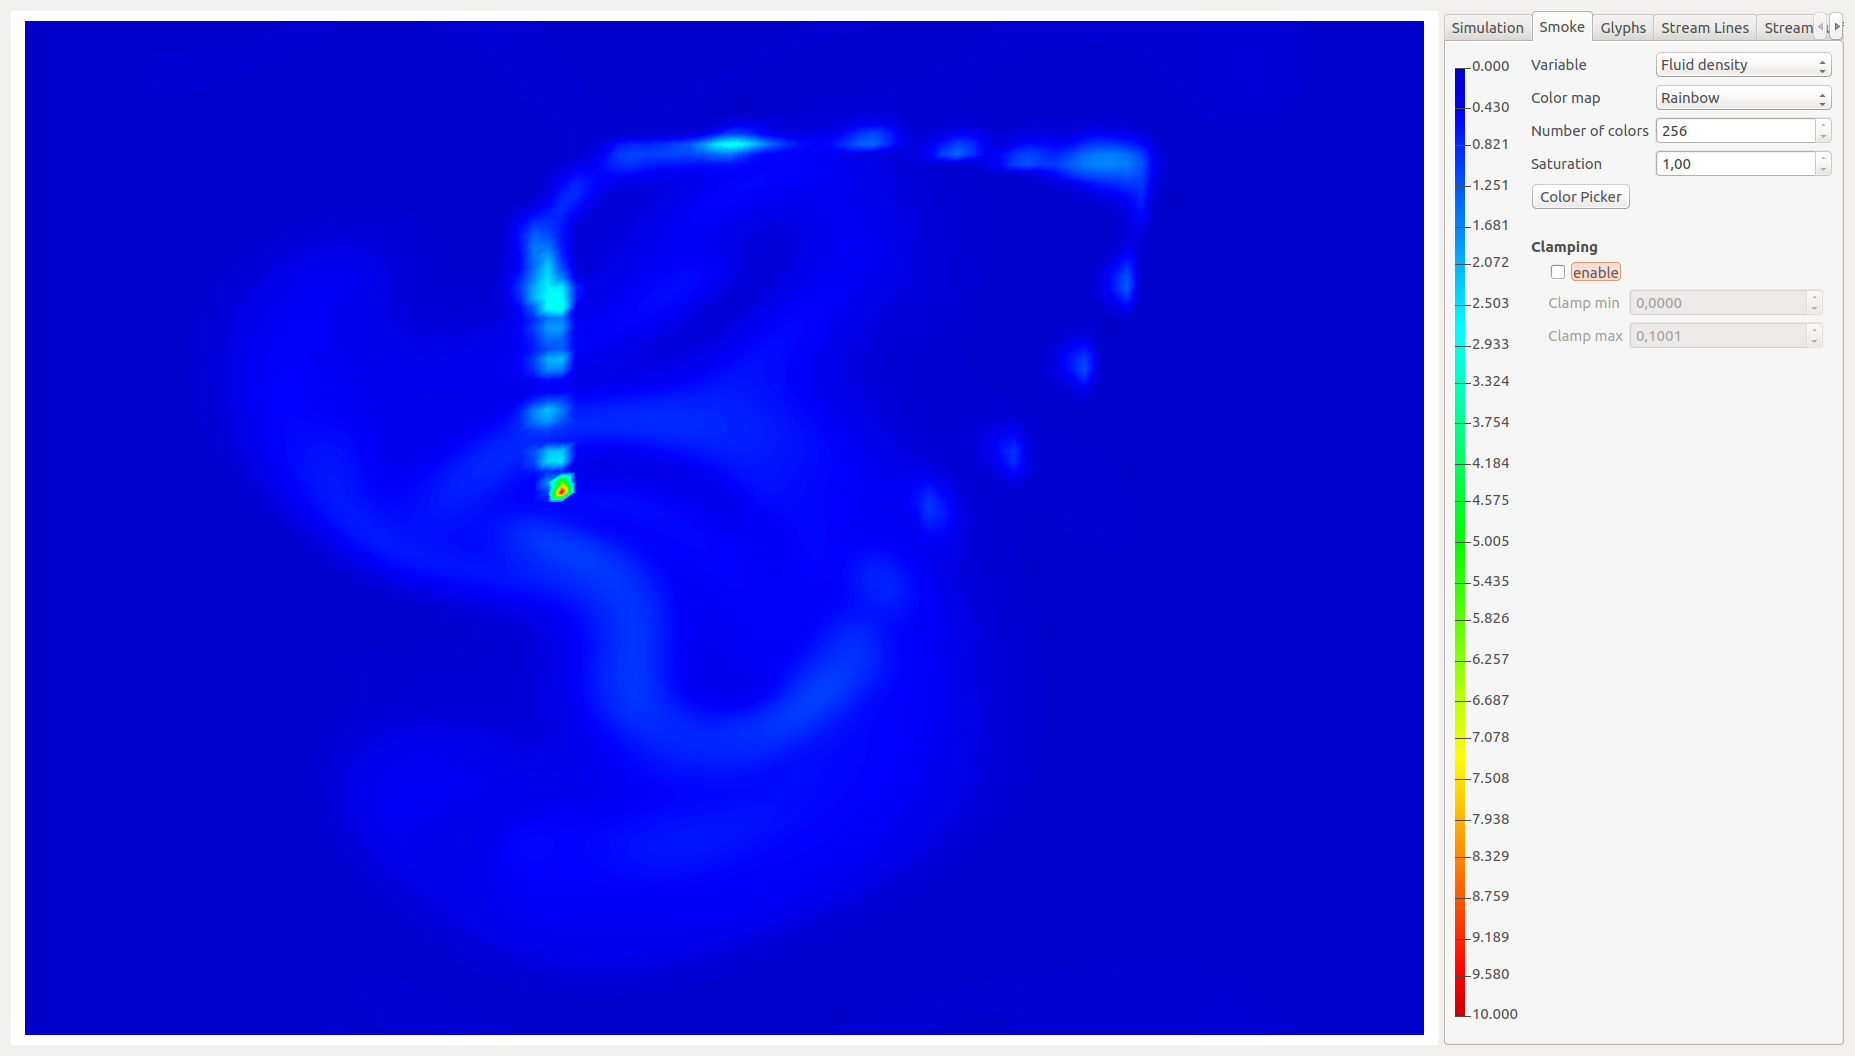
\includegraphics[width=\textwidth, trim={35px 30px 430px 30px}, clip]{colormapping/img/notclamped}
		\addrainbow{0.0}{10}
		\caption{no clamping}
		\label{fig:colormapping:clamped:disabled}
	\end{subfigure}
	\hspace{50px}
	\begin{subfigure}[t]{0.4\textwidth}
		\centering
		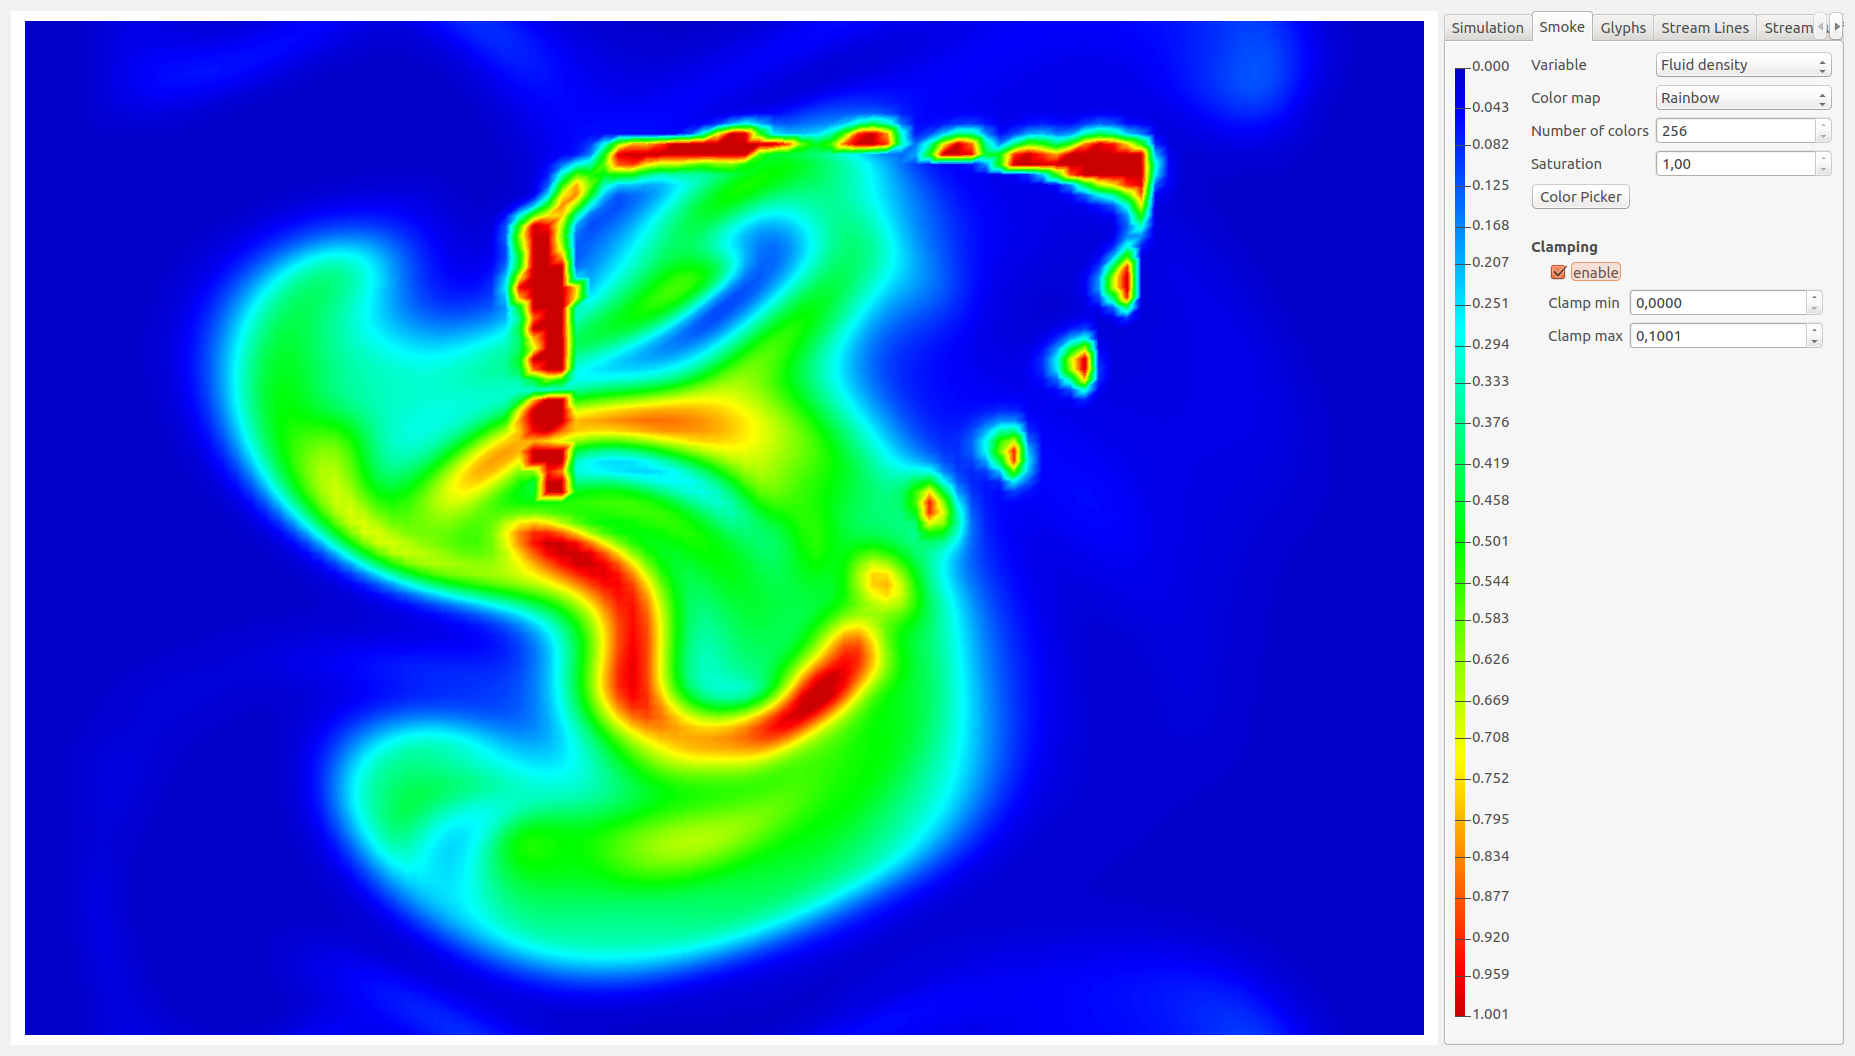
\includegraphics[width=\textwidth, trim={35px 30px 430px 30px}, clip]{colormapping/img/clamped_01}
		\addrainbow{0.0}{0.1}
		\caption{$[f^{clamp}_{min},\, f^{clamp}_{max}] = [0 \cdot f_{\text{min}},\, 0.1 \cdot f_{\text{max}}]$}
		\label{fig:colormapping:clamped:enabled}
	\end{subfigure}	
	\caption{Example of a visualization \subref{fig:colormapping:clamped:disabled} without and \subref{fig:colormapping:clamped:enabled} with clamping. The clamped version shows more detail, but does not distinguish scalar values above $0.1$. $[f_{\text{min}},\, f_{\text{max}}] = [0, 10]$.}
	\label{fig:colormapping:clamped}
\end{figure}